\chapter{Solution perspectives}\label{chap:chap4}

\section{Envisioned approach}

The scheme represented by the Figure \ref{fig:envision}, resumes the envisioned approach.

\begin{figure}[h]
	\begin{center}
		\leavevmode
		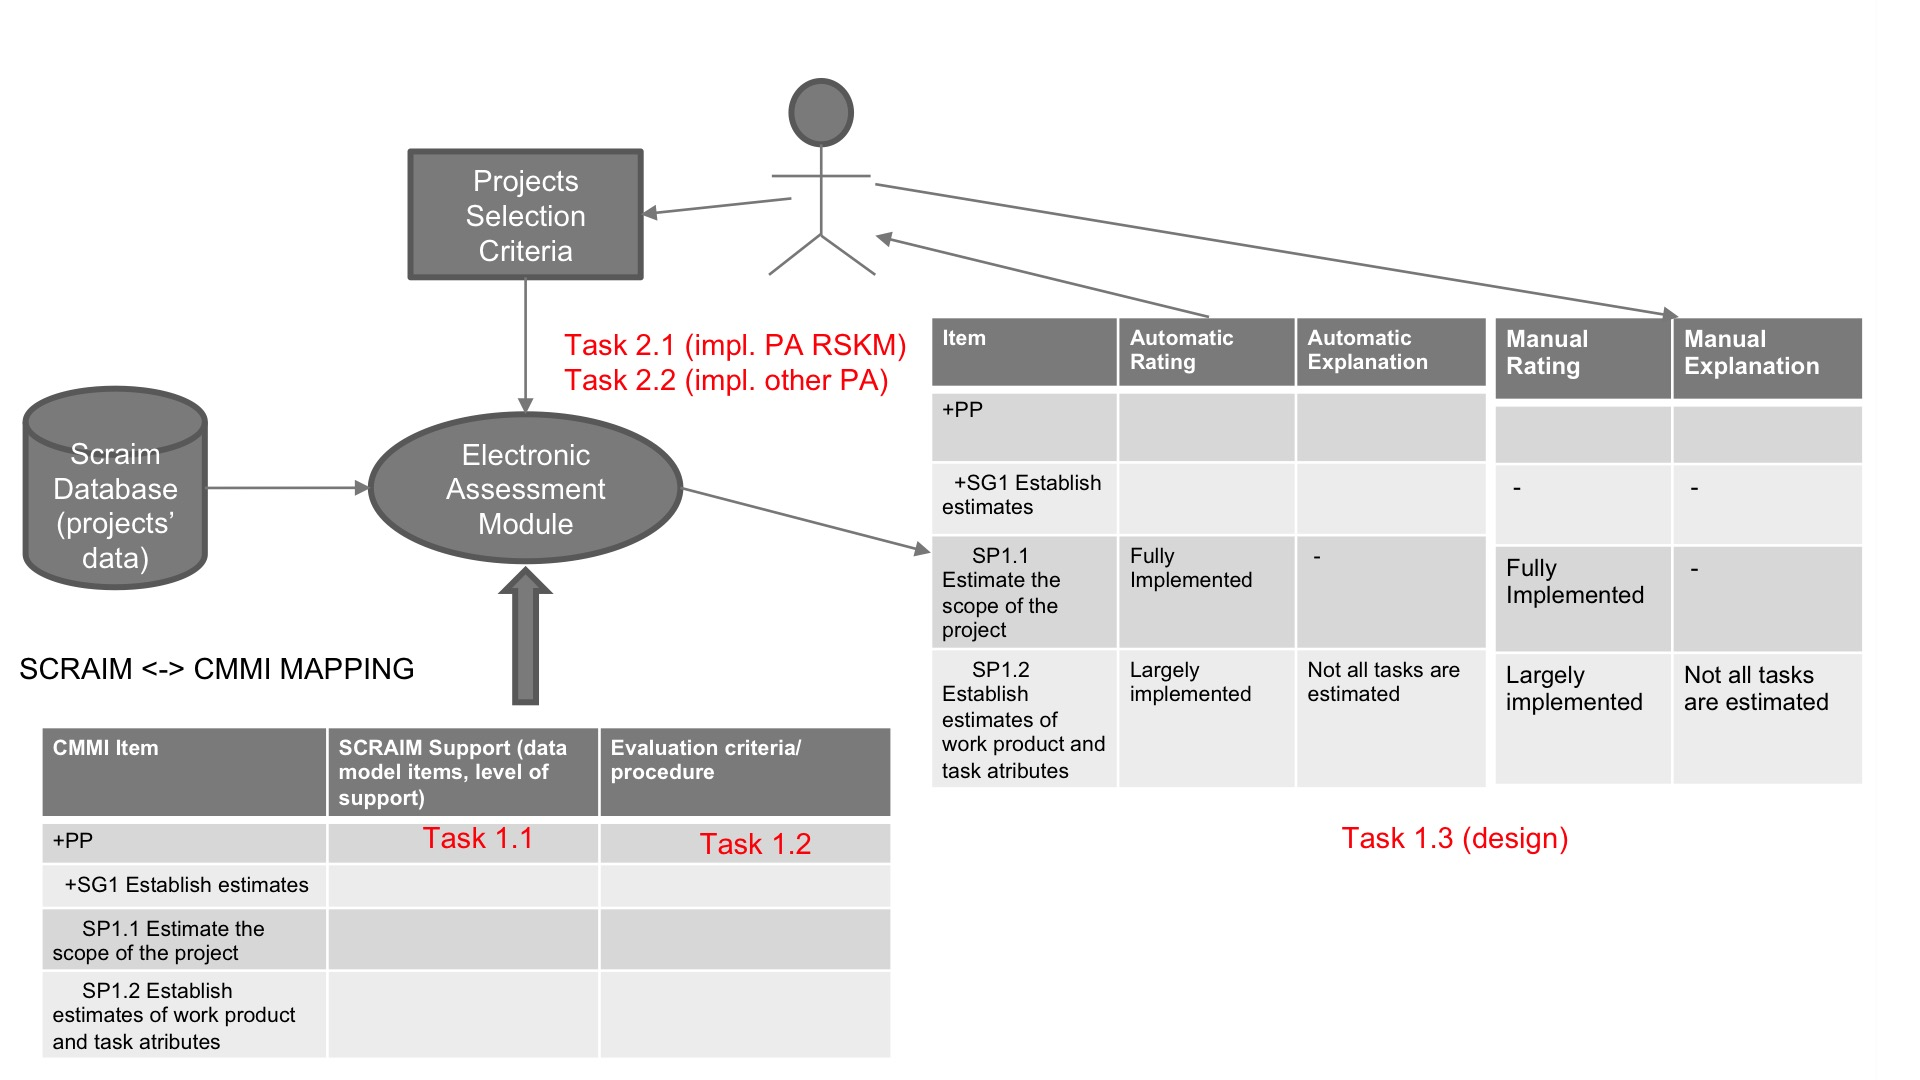
\includegraphics[width=1\textwidth]{envision}
		\caption{Envision approach scheme}
		\label{fig:envision}
	\end{center}
\end{figure}

The first step of this solution is to make a CMMI-SCRAIM mapping where it is going to be evaluated the data model items and the level of support available on SCRAIM and match them to CMMI best practices.

Then will be made the design of the module, where will be evaluated on a top level the data from SCRAIM database taking for base the previous mapping.

After completing these tasks will be evaluated the results obtained by this automatic rating and compared to manual ratings taking for base real projects selected from SCRAIM. 

For example in the Table \ref{tab:envision} its shown an automatic rating for the Project planning process area and the obtained explanation for that assessment. 


\begin{table}[h]
	\centering
	\caption{Automatic rating envision}
	\begin{tabular}{|p{6cm}|p{3cm}|p{3cm}|}
		\hline
		Item & Automatic Rating & Automatic Explanation\\
		\hline
		SG1 - Establish estimates&&\\
		SP 1.1 - Estimate scope of the project & Fully implemented & - \\
		SP 1.2 - Establish estimates of Work product and task attributes & Largely implemented & Not all tasks are estimated \\
		SP 1.3 - Define project lifecycle phases & Fully implemented & - \\
		SP 1.4 - Estimate effort and cost & Fully implemented & - \\
		\hline
		SG2 - Develop a project plan&&\\
		SP 2.1 - Establish the budget and schedule & Fully implemented & - \\
		SP 2.2 - Identify project risks & Partially implemented & Not all projects have risks identified \\
		SP 2.3 - Plan data Management & Fully implemented & - \\
		SP 2.4 - Plan the project's resources & Fully implemented & - \\
		SP 2.5 - Plan needed knowledge and skills & Fully implemented & - \\
		SP 2.6 - Plan stakeholder involvement & Not implemented & Not implemented \\
		SP 2.7 - Establish the project plan & Fully implemented & - \\
		\hline
		SG3 - Obtain commitment to the plan&&\\
		SP 3.1 - Review plans that affect the project & Fully implemented & - \\
		SP 3.2 - Reconcile work and resource levels & Fully implemented & - \\
		SP 3.3 - Obtain plan commitment & Largely implemented & Missing first meeting  \\
		\hline
	\end{tabular}
	\label{tab:envision}
\end{table}
\section{Work plan}

The work plan consists in four main tasks that are:
\begin{itemize}
	\item Conception - that contains the CMMI-SCRAIM mapping, definition of evaluation rules and user interface design.
	\item Implementation - consists in 6 iterations of one week each.
	\item Validation - analyze the results obtained by the module produced comparing to real assessments.
	\item Thesis and article writing
\end{itemize}

The Gantt of is presented on the Figure \ref{fig:workplan}.

\begin{figure}[h]
	\begin{center}
		\leavevmode
		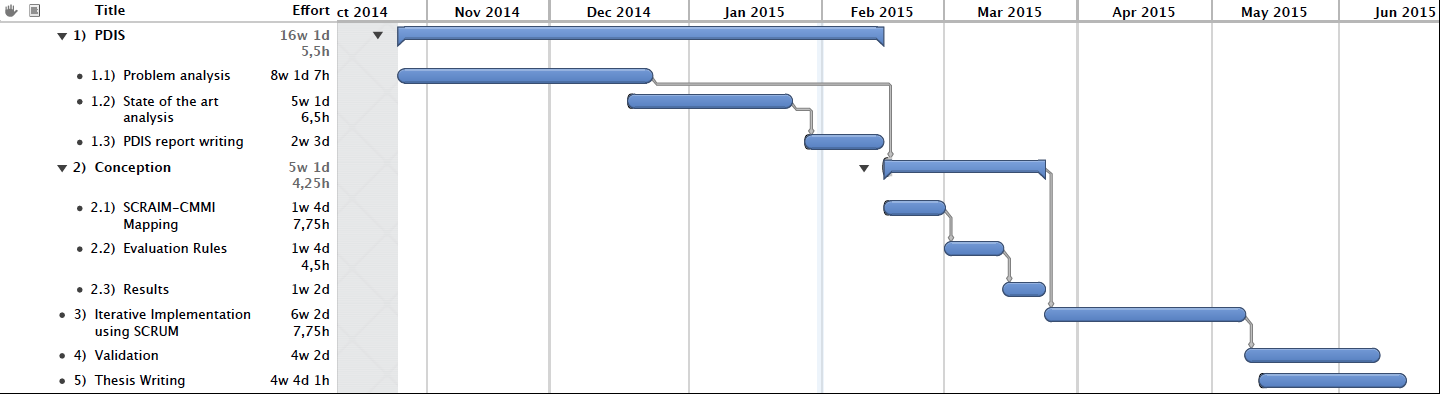
\includegraphics[width=1\textwidth]{workplan}
		\caption{Gantt Diagram}
		\label{fig:workplan}
	\end{center}
\end{figure}